\chapter{Background and Related Works}\label{chap:background}

\section{Vision Transformer}

\begin{figure}
	\centering
	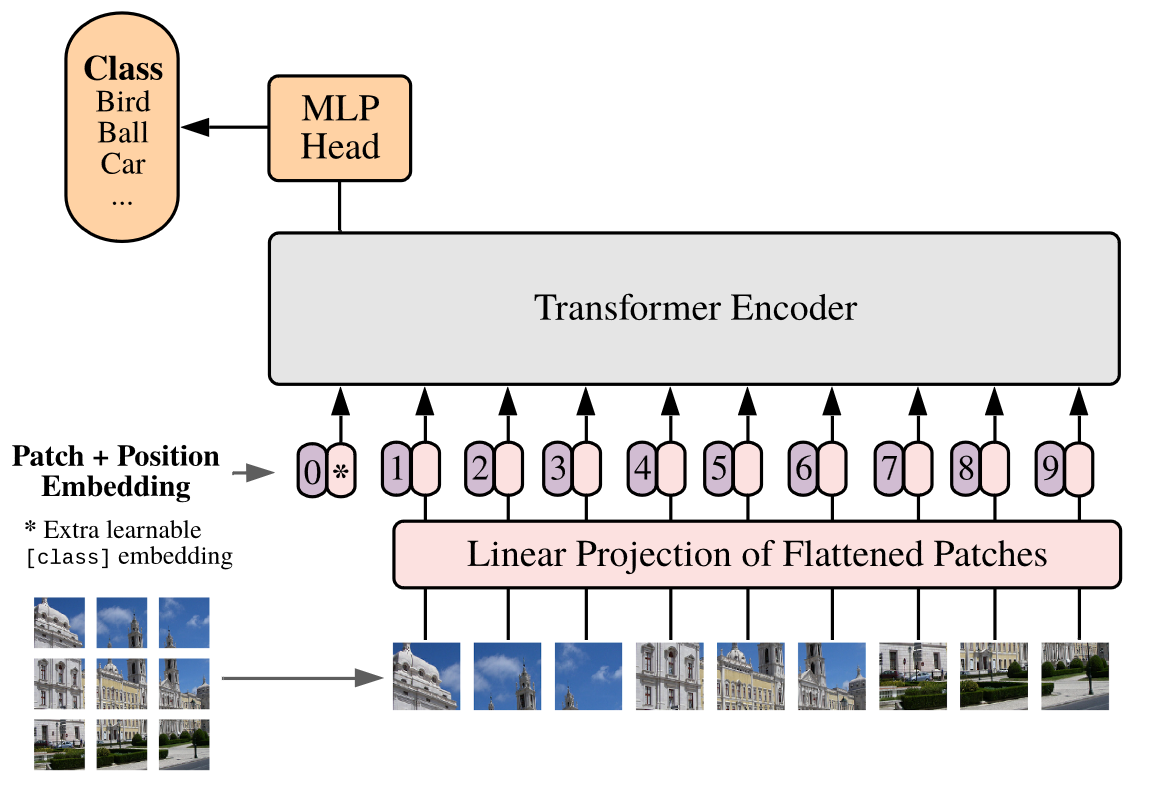
\includegraphics[width=0.9\textwidth]{Images/main/vit_full_arch.png}
	\caption[\textbf{ViT Architecture}]{\textbf{ViT Architecture}. ViT architecture from~\cite{dosovitskiy2020image}.}
	\label{fig:vit_full_arch}
\end{figure}

Vision Transformer (ViT), introduced by Dosovitskiy et al.~\cite{dosovitskiy2020image}, provides an alternative to Convolutional Neural Networks (CNNs) for image recognition, leveraging the transformer architecture to capture long-range dependencies and complex patterns that can complement and extend the capabilities of CNN-based models. The model applies Transformer architecture to image recognition tasks by treating image patches as sequences of tokens, akin to words in NLP. The highlight of the paper is reusing the transformer encoder from the revolutionary work Vaswani et al.~\cite{vaswani2023attentionneed} and adapting to use on images using patch tokenization and positional encoding.

As CutLER uses the features from a self-supervised ViT to generate masks, it is crucial to understand the basics architecture and working of ViT to get a complete picture of the feature generation process. Figure \ref{fig:vit_full_arch} shows the complete architecture of ViT. We are going to go into the main parts of the architecture for a better understanding of the process.

\subsection{Patch Tokens and Positional Encoding}

As each input is an image, unlike sequence of words or tokens in~\cite{vaswani2023attentionneed}, the image is divided in fixed size patches (16x16 or 8x8) and each patch is treated as a token and each token is embedded into a fixed-dimensional vector using a learned embedding layer.

\begin{equation}
	\label{eq:pos_encoding}
	z⁰_i = z_i + p_i
\end{equation} 

For each token, instead of using sinusoidal position encodings~\cite{vaswani2023attentionneed} to retain information about the position of tokens in the sequence, a learnable position embedding is added as shown in the Eq.~\ref{eq:pos_encoding}, where \(p_i \in \mathbb{R}^{D}\) is the learnable position embedding for patch i. 

\begin{equation}
	\label{eq:full_pos_encoding}
	Z = [z_{class}; z⁰_1; z⁰_2;...; z⁰_N]
\end{equation}

Apart from \cite{vaswani2023attentionneed}, ViT~\cite{dosovitskiy2020image} introduces a special classification token \(z_{class}\) which is prepended to the sequence of patch embeddings. This token aggregates information from all patches and is used for the final classification task. The final encoding look like Eq.~\ref{eq:full_pos_encoding}.

\subsection{Transformer Encoder}
The sequence of patch embeddings, augmented with positional information, is processed by the Transformer encoder. The encoder consists of multiple layers, each comprising Multi-Head Self-Attention (MSA) and Multi-Layer Perceptrons (MLPs), with Layer Normalization (LN) and residual connections. A weighted average~\cite{weng2020transformer} of individual attention outputs constitute the final output. Figure~\ref{fig:transformer_encoder} illustrates the architecture of the transformer encoder. We briefly look into each part.

\begin{figure*}
	\centering
	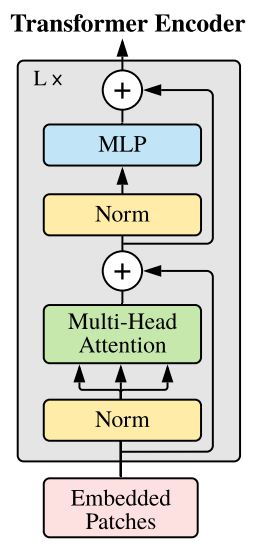
\includegraphics[width=0.3\textwidth]{Images/main/transformerblock.png}
	\caption[\textbf{Transformer Encoder Architecture}]{\textbf{Transformer Encoder Architecture}. Illustration of the Transformer encoder architecture in ViT~\cite{dosovitskiy2020image}.}
	\label{fig:transformer_encoder}
\end{figure*}

\subsubsection{Multi-Head Self-Attention (MSA)}
Self-attention allows the model to weigh the importance of different patches relative to each other.

\begin{subequations}
	\label{eq:qkv}
	\begin{align}
		\text{Queries  } Q = zW^{Q}_i \label{eq:query} \\
		\text{Keys  } K= zW^{K}_i \label{eq:key} \\
		\text{Values  } V = zW^{V}_i \label{eq:value}
	\end{align}
\end{subequations}

Given that \(d_k\) is the dimensionality of the key, query, and value vectors and \(W^Q_i, W^K_i, W^V_i \in \mathbb{R}^{D \times d_k }\) are learnable weight matrices, query, key, and value are computed as given in Eq.~\ref{eq:qkv}.


For each attention head \(i\),
\begin{equation}
	head_i =
	\text{Attention  }(Q_i,K_i,V_i) = \text{softmax  } \left(\frac{Q_iK^{T}_i}{\sqrt{d_k}}\right)V_i
\end{equation}

The outputs from all heads are concatenated and linearly transformed. Given \(W^O \in \mathbb{R}^{h-d_k \times D } \):
\begin{equation}
	MSA(z) = \text{Concat  }(head_i, head_2..., head_h)W^O
\end{equation}

\subsubsection{Layer Normalization and Residual Connections}
Each layer in the Transformer encoder includes Layer Normalization (LN) and residual (skip) connections
\begin{equation}
	z' = \text{MSA}(\text{LN}(z)) + z
\end{equation}
\begin{equation}
	z'' = \text{MLP}(\text{LN}(z')) + z'
\end{equation}
The Multi-Layer Perceptron (MLP) usually consists of two linear transformations with a GELU non-linearity in between. Assuming \(W_1\) ans \(W_2\) are learnable weight matrices:
\begin{equation}
	\text{MLP}(x) = W_2(\text{GELU}(W_1x))
\end{equation}

\subsubsection{Output Layer}
The final output of the classification token is passed through a linear layer to produce the classification logits. Given \(C\) is the number of classes and \(W_{class} \in \mathbb{R}^{C \times D }\):
\begin{equation}
	\text{logits} = W_{class} \text{ }.\text{ } z''_{class}
\end{equation}
The linear layer projects the final representation of the classification token into the space of class labels.

\section{Self-Supervised Feature Learning}
Self-supervised feature learning is a crucial process that identifies patterns within extensive unlabeled datasets without the need for human-annotated labels. Plenty of research has been done in this field in the recent years. Several methods have been proposed, each with unique mechanisms and varying levels of success.

\subsection{Contrastive Learning}
Contrastive learning has gained significant attention for its effectiveness in self-supervised feature learning. One of the seminal works in this area is SimCLR~\cite{chen2020simple}, It employs a simple yet robust framework that leverages data augmentations to create positive pairs from the same image and negative pairs from different images. The model uses a contrastive loss to distinguish between these pairs, learning robust representations in the process. On the other hand, MoCo (Momentum Contrast)~\cite{he2020momentum} introduces a dynamic dictionary with a momentum encoder. This approach allows the model to maintain a queue of negative samples, effectively reducing memory requirements and improving scalability. Nevertheless, it still requires a substantial number of negative samples to function optimally and necessitates careful tuning of the momentum parameter to balance stability and learning efficiency.

\subsection{Clustering-Based Feature Learning}
Clustering-based feature learning approaches automatically uncover the natural groupings of data within the latent representation space. This clustering process helps in understanding the inherent structure of the data by grouping similar data points together based on learned features. Agglomerative Clustering with Self-supervision~\cite{asano2020selflabelling} can capture multi-scale structures and found to be effective for diverse datasets. But found to be computationally expensive and needs careful tuning of the self-supervised task. SwAV~\cite{caron2021unsupervised} combines clustering with contrastive learning by swapping assignments between different augmented views of the image. This method is efficient in terms of computational resources and achieves state-of-the-art performance on several benchmarks. But it is sensitive to the choice of hyperparameters.

\subsection{Distillation-Based Methods}
Distillation-based methods have also shown considerable promise in self-supervised learning. BYOL (Bootstrap Your Own Latent)~\cite{grill2020bootstrap} introduces a teacher-student network where the student learns to predict the teacher's representations. Remarkably, BYOL achieves this without using negative samples, simplifying the training process and reducing computational demands. However, it is sensitive to the choice of data augmentations and network architecture, and there is a potential risk of model collapse if not properly tuned. DINO~\cite{caron2021emerging}, extends the self-distillation approach to Vision Transformers~\cite{dosovitskiy2020image}. DINO captures global image representations effectively without relying on negative samples. It shows strong performance on object detection and segmentation tasks, showcasing the potential of transformers in self-supervised learning.

Unlike traditional unsupervised representation learning methods that focus primarily on learning generalized visual features, our research centers on CutLER~\cite{wang2023cut}, which leverages these learned features, specifically DINO~\cite{caron2021emerging}, to focus on the task of instance detection. While CutLER builds upon the robust feature representations provided by DINO, it further enhances performance through advanced techniques and refinements.

\section{DINO}
The self-supervised model DINO, introduced by Caron, Mathilde, et al.~\cite{caron2021emerging}, achieves remarkable performance that rivals many state-of-the-art CNNs trained with supervision. DINO stands out for its ability to extract features that reveal clear information about semantic segmentation and scene layout within images. This capability distinguishes DINO from supervised ViTs and ConvNets, underscoring its potential for sophisticated computer vision tasks without relying on annotated data.

As we will be using DINO features for producing the pseudo masks in CutLER~\cite{wang2023cut}, we need a basic understanding of DINO architecture and training.

\subsection{Knowledge Distillation}
 Knowledge distillation plays a crucial role in training a student model to mimic the behavior and representations learned by a teacher model, both of which are ViTs. 
 
\begin{figure*}
	\centering
	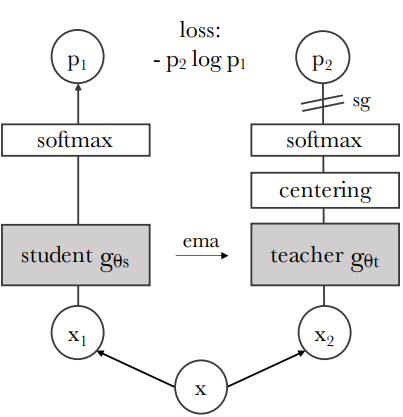
\includegraphics[width=0.5\textwidth]{Images/main/dino.png}
	\caption[\textbf{DINO Architecture }]{\textbf{Architecture of DINO} Illustration provided in~\cite{caron2021emerging}.}
	\label{fig:dino}
\end{figure*} 
 
 Initially, the teacher model is typically a ViT that is pre-trained on a large dataset using self-supervised learning techniques. The teacher captures rich, generalized features from the data. The student model is a smaller ViT that aims to replicate the teacher's performance but with fewer parameters, making it computationally lighter and potentially faster during inference.
 
\subsubsection{Momentum Encoder for Teacher}
Instead of using the teacher model directly, DINO employs a momentum encoder mechanism for stability and improved generalization. This means that the parameters of the teacher model are updated using a moving average of the student model's parameters, rather than directly during training.
\begin{equation}
	\label{eq:momentum}
	\theta_t \leftarrow m \theta_t + (1 - m) \theta_s
\end{equation}
The teacher model's parameters are updated using a momentum update rule as given in Eq.~\ref{eq:momentum}. Where \(\theta_t\) are the parameters of the teacher model, \(\theta_s\) are the parameters of the student model, and \(m\) is a momentum parameter (typically close to 1) that controls the rate of updating.

\subsection{Training Process}
DINO uses different augmentations of the same image to create multiple views. These augmented views are passed through both the teacher and student models. Outputs from both models are projected into a lower-dimensional space using projection heads. Outputs from both models are projected into a lower-dimensional space using projection heads. The optimization objective is to minimize the cross-entropy loss between the predicted probability distributions of the teacher and student models. Assume \(P_t(x)\) and \(P_s(x)\) represent the probability distributions predicted by the teacher and student models, respectively. The training process is illustrated in~\ref{fig:dino}

\begin{equation}
	\label{eq:dino_objective}
	\min_{\theta_s} \mathcal{H}(P_t(x), P_s(x))
\end{equation}

The cross-entropy loss is computed between the softened distributions of the teacher and student models across all augmented views as given in Eq.~\ref{eq:dino_objective}.


\section{Unsupervised Object Detection and Instance Segmentation}
If we consider the recent methods for unsupervised object detection semantic segmentation, most of them leverage on self-supervised Vision Transformer (ViT)~\cite{dosovitskiy2020image} features. In DINO~\cite{caron2021emerging} it is observed that the underlying semantic segmentation of images can be extracted using the saliency maps from the ViT. 

The quality of this segmentation is superior to the existing methods if the image contains only is one instance. The superiority of DINO features to separate foreground and background has been affirmed by later works~\cite{engstler2023understanding}. Building on this observation, both LOST ~\cite{simeoni2021localizing} and TokenCut~\cite{wang2022tokencut} utilize DINO features to segment a single salient object from each image. These methods capitalize on the strength of DINO to construct a graph from the features of image patches. Unlike TokenCut and DINO, which can only detect one instance, LOST is capable of finding multiple instances within an image. But it can't be used as a pre-trained model for down stream tasks. But CutLER~\cite{wang2023cut} not only can detect multiple instances, the model can be further used as a pretrained model for label-efficient and fully-supervised learning.

MaskDistill~\cite{vangansbeke2022discovering} advocate a data-driven approach to mine object masks via self-supervised vision transformers and distill multiple object masks per image via an object segmentation model (Mask R-CNN). Then a final segmentation model is trained using the found object masks. Even though MaskDistill produces similar quality masks compared to MaskCut, as it only produces one class agnostic mask per image and MaskCut produces up to N number of masks per image to use as pseudo labels, MaskCut weighs over MaskDistill in quantity.

FreeSOLO~\cite{wang2022freesolo} and the follow up work Exemplar-FreeSOLO~\cite{Ishtiak_2023_CVPR} (with its addition of a randomly drawn pool of exemplars used in a contrastive learning loss) generates coarse segmentation masks with low guality and refines it further through self training similar to CutLER. But the poor quality of the coarse maps is a major draw back of this method, where as CutLER masks made by the MaskCut~\cite{wang2023cut, wang2022tokencut} algorithm are usually better in quality and quantity than the initial masks used by MaskDistill~\cite{vangansbeke2022discovering} and FreeSOLO~\cite{wang2022freesolo}. 

As CutLER outperforms other methods in most cases, including producing better pseudo ground truth masks, ability to detect multiple instances, compatibility with various detection architectures, usable as pretrained model for supervised detection, our work would mostly focus on studying and improving the performance of CutLER.

\section{CutLER}
\begin{figure}
	\centering
	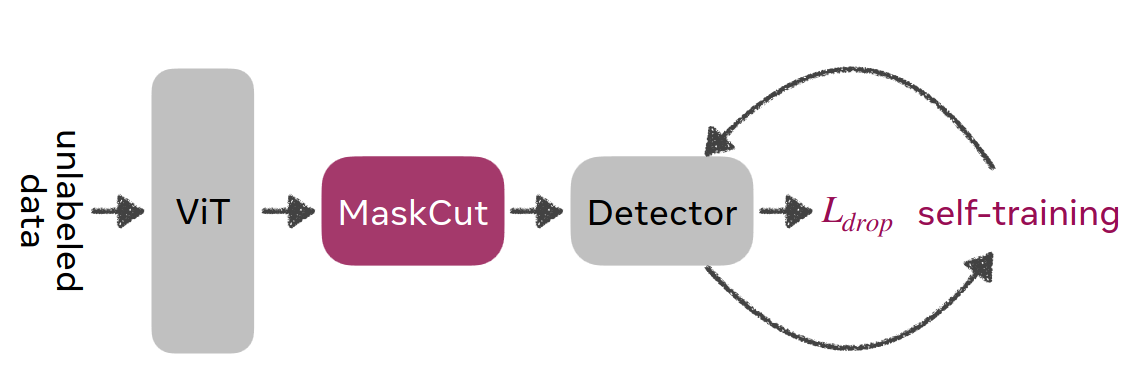
\includegraphics[width=0.8\textwidth]{Images/main/cutler_flow.png}
	\caption[\textbf{CutLER Overview}]{\textbf{CutLER overview} The flow consist of MaskCut for extracting coarse masks from the features of a self-supervised ViT. Following this, a detector utilizing a loss dropping strategy designed to be resilient against objects that MaskCut may overlook is used. Additionally, the model undergoes further enhancement through multiple rounds of self-training. Illustration taken from~\cite{wang2023cut}}.
	\label{fig:cutler_flow}
\end{figure} 

CutLER~\cite{wang2023cut} introduces a novel approach to address the challenges of object detection and instance segmentation in an unsupervised learning framework. By integrating Copy-Paste~\cite{ghiasi2021simplecopypastestrongdata} augmentation and a contrastive learning framework, the method not only circumvents the need for labeled data but also achieves state-of-the-art results in object detection and instance segmentation. The complete process is illustrated in Fig. \ref{fig:cutler_flow}.
 
\subsection{Normalized Cut}
Normalized Cut (NCut)~\cite{normcut} is a graph cut method where goal is to partition an image into segments (or regions) by cutting a graph that represents the image, such that the similarity within each segment is maximized while the dissimilarity between different segments is also maximized. Understanding the NCuts algorithm is crucial, as CutLER's pseudo-ground truth masks rely on repeated NCuts to generate accurate masks. This process is key to CutLER's improved performance in unsupervised instance detection and segmentation.

In Normalized Cut, an image is represented as an undirected graph \( G = (V, E) \), where \( V \) is the set of nodes, each representing a pixel or a group of pixels and \( E \) is the set of edges, each representing a connection between two nodes, with weights \( w(i, j) \) indicating the similarity between nodes \( i \) and \( j \). A basic cut is defined as the sum of the edge weights that are severed by the partition. A basic Cut is defined as the sum of the edge weights that are severed by the partition as given in Eq.~\ref{eq:cut}:

\begin{equation}
	\label{eq:cut}
	\text{Cut}(A, B) = \sum_{i \in A, j \in B} w(i, j)
\end{equation}

However, minimizing the cut alone tends to produce small, isolated segments. To address this, the Normalized Cut criterion is introduced. The Normalized Cut is defined as follows:

\begin{equation}
	\label{eq:norm_cut}
	\text{Ncut}(A, B) = \frac{\text{Cut}(A, B)}{\text{Assoc}(A, V)} + \frac{\text{Cut}(A, B)}{\text{Assoc}(B, V)}
\end{equation}

where \( \text{Assoc}(A, V) = \sum_{i \in A, j \in V} w(i, j) \) is the total connection from nodes in \( A \) to all nodes in the graph. The goal is to find the partition \( (A, B) \) that minimizes the NCut value. This can be expressed as an eigenvalue problem. The solution involves finding the eigenvector corresponding to the second smallest eigenvalue of the generalized eigenvalue problem given as Eq.~\ref{eq:eig_problem}.

\begin{equation}
	\label{eq:eig_problem}
	(D - W)x = \lambda D x
\end{equation}

where \( d(i) = \sum_{j} w(i, j) \) is the degree of node \( i \), and \( D \) is a diagonal matrix with \( d(i) \) on the diagonal and \( W \) be the weight matrix of the graph. The resulting eigenvector is used to partition the graph by thresholding its values.

\subsection{TokenCut}
TokenCut~\cite{wang2022tokencut} builds on the principles of Normalized Cut but adapts them to work within the framework of ViTs. Instead of operating on pixels, TokenCut segments an image by working with tokens - image patches processed by a ViT. In TokenCut, each token is treated as a node in a graph, and the edges are defined by the self-attention scores from the transformer, which capture the affinity between tokens. The goal remains similar: to partition the graph of tokens in a way that minimizes the NCut criterion. By leveraging the transformer’s attention mechanism, TokenCut can effectively capture global dependencies and segment objects in a self-supervised manner, even without labeled data. However, TokenCut only produces one mask per image, which limits the method from detecting multiple objects in an image. This issue is addressed in MaskCut.

\subsection{MaskCut}
\begin{figure}
	\centering
	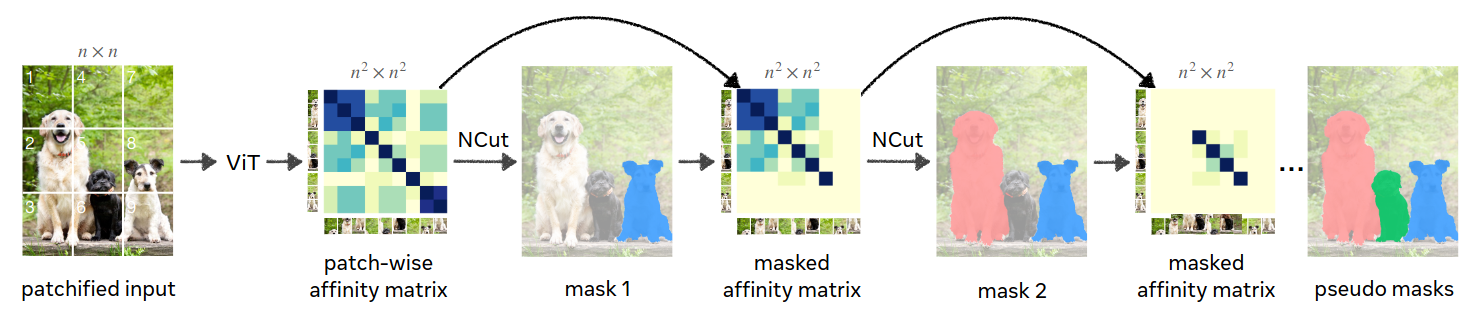
\includegraphics[width=1.0\textwidth]{Images/main/maskcut_eg.png}
	\caption[\textbf{MaskCut Flow}]{\textbf{MaskCut} works on the patch-wise
		similarity matrix for the image using a self-supervised DINO~\cite{caron2021emerging} model feature. N=3 defines the number of times NCut~\cite{normcut} is repeated on the background. In this case, 3 instances will be discovered per image in each step. Illustration taken from~\cite{wang2023cut}}.
	\label{fig:maskcut_flow}
\end{figure}

Like TokenCut~\cite{wang2022tokencut}, MaskCut considers image segmentation problem as a graph partitioning task~\cite{normcut}. The nodes are tokens (each representing an image patch) and edges connect every pair of nodes, with weights \(W_{ij}\) reflecting the similarity between tokens. The optimization problem reduces the cost of dividing the graph into two sub-graphs, or a bipartition, by solving a generalized eigenvalue problem as given in Eq.~\ref{eq:eig_problem}. 

The similarity weight \( W_{ij} \) of NCut in TokenCut based on the similarity of patches in the DINO feature space. Following recent methods~\cite{simeoni2021localizingobjectsselfsupervisedtransformers, vangansbeke2022discoveringobjectmaskstransformers, wang2023tokencutsegmentingobjectsimages}, they specifically employ the cosine similarity of 'key' features from the final attention layer of the DINO-pretrained model, represented as:

\begin{equation}
W_{ij} = \frac{K_i \cdot K_j}{\|K_i\|_2 \|K_j\|_2}
\end{equation}

where \( K_i \) denotes the 'key' feature of patch \( i \). They then solve Eq.~\ref{eq:eig_problem} to find the second smallest eigenvector \( x \). The main drawback of TokenCut is that it only uses the smallest eigenvector resulting in finding only one instance in the image. MaskCut overcomes this drawback and finds more instances by iteratively applying the same process in the background N times as given in Fig.~\ref{fig:maskcut_flow}. The figure shows the flow of MaskCut algorithm for N=3 (Defines the number of times NCut is repeated. In this case, 3 instances will be discovered per image) Building on the work of~\cite{wang2023tokencutsegmentingobjectsimages, caron2021emergingpropertiesselfsupervisedvision}, a patch-wise similarity matrix for the image using features from a self-supervised DINO model~\cite{caron2021emerging} is created. Normalized Cuts~\cite{normcut} is applied to this matrix to obtain a single foreground object mask for the image. Subsequently, this foreground mask is used to mask out the affinity matrix values and repeat the process. This iterative approach enables MaskCut to identify multiple object masks within a single image.

MaskCut uses two conditions to improve the performance.
\begin{enumerate}
	\item An object centric prior~\cite{obj_centric_prior} is used to filter out backgrounds. ie, if the foreground contains more than 2 out of 4 corners, foreground and background are switched.
	
	\item From the intuition that foreground patches are more prominent than background ones~\cite{caron2021emergingpropertiesselfsupervisedvision, cond1_support_2}, we assert that foreground mask should contain the patch corresponding to the maximum absolute value in the second smallest eigenvector.
\end{enumerate}
  If condition 1 is not satisfied and current foreground contains two corners, background and foreground are switched.

\subsection{DropLoss}
A standard detection loss penalizes predicted regions \( r_i \) that do not overlap with the 'ground truth'. Since the ground truth masks from MaskCut may miss some instances, the standard loss does not allow the detector to identify new instances not labeled in the ground truth. To address this, the author proposes ignoring the loss for predicted regions \( r_i \) with minimal overlap with the ground truth.

\begin{equation}
	\label{eq:drop_loss}
L_{\text{drop}}(r_i) = \mathds{1}(\text{IoU}_i^{\text{max}} > \tau^{\text{IoU}}) L_{\text{vanilla}}(r_i)
\end{equation}

Specifically, during training, the loss is dropped for any predicted region \( r_i \) that has a maximum overlap of \( \tau^{\text{IoU}} \) with any ground truth instance as given in Eq. \ref{eq:drop_loss} where \(\text{IoU}_i^{\text{max}}\) denotes the maximum IoU with all ground truth for \( r_i \), and \( L_{\text{vanilla}} \) refers to the standard loss function for detectors. \( L_{\text{drop}} \) avoids penalizing the model for detecting objects missed in the 'ground truth', thus encouraging the exploration of different image regions.

\begin{figure}
	\centering
	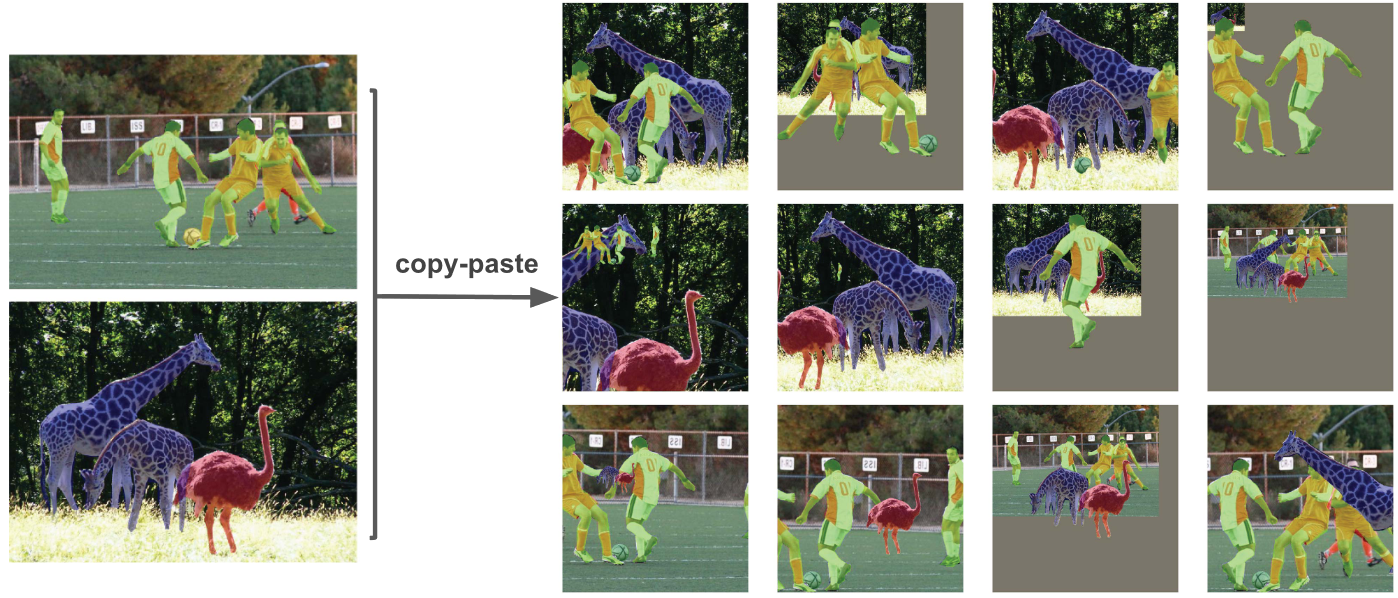
\includegraphics[width=1.0\textwidth]{Images/main/copy-paste.png}
	\caption[\textbf{Copy-Paste Augmentation}]{Illustration of Copy-Paste augmentation from~\cite{ghiasi2021simplecopypastestrongdata}}.
	\label{fig:copy_paste_aug}
\end{figure}

\subsection{Copy-Paste Augmentation}
Copy-Paste Augmentation~\cite{ghiasi2021simplecopypastestrongdata} is a data augmentation technique used to enhance the diversity of training datasets by artificially creating new training samples. This method involves copying objects from one image and pasting them onto another, thereby generating new training examples with diverse object placements and backgrounds as illustrated in Fig.~\ref{fig:copy_paste_aug}. The pasted objects can be resized, rotated, or otherwise manipulated to fit the new context. Lastly, the ground-truth annotations are also adjusted accordingly

In Cutler, instead of using the standard copy-paste augmentation, where masks are rescaled with a factor between 0.8 and 1.25, masks are randomly downsampled with a scalar uniformly sampled between 0.3 and 1.0. This approach enables Cutler to recognize even smaller instances in the image effectively.

\subsection{Training}
The training process is divided into two stages: initial training followed by self-training, as depicted in Fig.\ref{fig:cutler_flow}. CutLER is agnostic regarding the choice of detector, allowing the use of any preferred detector. However, based on the experiments detailed in the paper, Cascade Mask R-CNN\cite{cai2019cascadercnnhighquality} yields better results compared to Mask R-CNN~\cite{he2018maskrcnn}.

First, pseudo-ground truth masks are generated using MaskCut for all images in Imagenet~\cite{deng2009imagenet} training set. The detector with a ResNet-50~\cite{he2015deepresiduallearningimage} backbone is trained using these pseudo-ground truth masks for 160K iterations with Copy-Paste augmentations and DropLoss.

\subsubsection{Self-Training}
To further improve the model performance, several self-training loops are also carried out. The CutLER mask predictions of each image with confidence score > 0.7 generated using the final model of last training phase and corresponding MaskCut masks which doesn't overlap more than 50\% with the predicted masks together forms the pseudo-ground truth masks for the first round of self-training. The same process is repeated for the following self-training rounds except that instead of MaskCut masks, pseudo-ground truth masks of the previous stage is used to compare with predicted masks. Each self training round is consist of 80K rounds and does not use DropLoss as we obtain comparatively good quality masks in the first round it self. The detailed information about the training are explained later in Section~\ref{section:implementation_details}.

\subsection{Mask Refinement in CutLER}
The presence of incorrect masks in pseudo-ground truth can lead to overfitting on incorrect patterns or failure to generalize properly across different instances. To mitigate these issues, techniques like iterative refinement, robust loss functions, and the incorporation of consistency constraints have been proposed. Tang et al.~\cite{Tang_2018_CVPR} and Wang et al.~\cite{ziegler2022selfsupervisedlearningobjectparts} explore these approaches. 

Iterative refinement helps in progressively reducing this noise, leading to cleaner and more reliable labels~\cite{xie2020selftrainingnoisystudentimproves}. Popular refinement methods incorporate strategies like thresholding, where only high-confidence predictions are used for retraining, or use ensemble methods to combine predictions from multiple models for more reliable masks. CutLER also uses this approach.

In CutLER, Before each self-training loop, 30 masks per image are generated for the entire Imagenet dataset using the latest trained model. Of these, masks are filtered based on the confidence score. In the paper, the masks with confidence score greater than \(0.7 - 0.05 * i\) on the \(i\) th iteration are kept and the rest are rejected. These filtered CutLER masks are compared with the corresponding MaskCut masks (in the first self-training round) or the pseudo-ground truth masks from the last round for each image. If the IoU between CutLER mask and MaskCut mask is less than 0.5, the corresponding MaskCut mask is added along with CutLER masks and this constitutes the pseudo-ground truth for the self-training loop.

The intuition is to retain masks from previous pseudo-ground truths that do not significantly overlap (i.e., overlap less than 0.5) with the current predictions. This strategy allows CutLER to explore new regions of the image that have not been thoroughly examined in previous iterations. However, a challenge with this approach is that it may perpetuate the inclusion of noisy masks in the ground truth during each self-training loop. Our approach seeks to address this issue by implementing a more refined method for removing the noisy background masks from the MaskCut masks and to improve the quality of the masks iteratively.